%        File: Intro.tex
%     Created: Sun Mar 02 03:00 PM 2014 P
% Last Change: Sun Mar 02 03:00 PM 2014 P
%
\documentclass[titlepage,letterpaper,12pt]{article}
\usepackage[sorting=none,backend=bibtex]{biblatex}
\usepackage{fullpage}
\usepackage{hyperref}
\hypersetup{colorlinks=true,urlcolor=blue}
\usepackage[all]{hypcap}
\usepackage{amsmath}
\usepackage{graphicx}
\usepackage[font=small,labelfont=bf]{caption}
%\usepackage[doublespacing]{setspace}
\usepackage[onehalfspacing]{setspace}
\addbibresource{CapstoneCitations.bib}

\pagestyle{plain}

\title{Humanoid Robotic Subsystems}
\date{April 14, 2014}
\author{Wenbo Wang \\University of California, Berkeley}

\begin{document}

\begin{titlepage}
\begin{center}

% Upper part of the page. The '~' is needed because \\
% only works if a paragraph has started.

    \textsc{\large University of California, Berkeley College of Engineering}\\[0.5cm]
    \textsc{\Large MASTER OF ENGINEERING - SPRING 2014}\\[1.5cm]

    \textsc{\large Electrical Engineering and Computer Sciences}\\[0.5cm]
    \textsc{\LARGE Humanoid Robotics Subsystems}\\[0.5cm] 
    \textsc{\LARGE Wenbo Wang}\\[1.5cm]

\end{center}

\begin{flushleft}
{
    This Masters Project Paper fulfills the Master of Engineering degree
    requirement\\[0.5cm]
    Approved by:\\[0.5cm]
    1.  Capstone Project Advisor: \\[0.5cm]
    Signature: \underline{\hspace{7cm}} Date \underline{\hspace{3cm}}\\[0.5cm]
    Print Name: Donald Wroblewski\\
    Department: Fung Institute\\[1.5cm]

    2. Faculty Committee Member \#2: \\[0.5cm]
    Signature: \underline{\hspace{7cm}} Date \underline{\hspace{3cm}}\\[0.5cm]
    Print Name: Ruzena Bajcsy\\
    Department: Electrical Engineering and ComputerSciences\\
}
\end{flushleft}

\end{titlepage}


\begin{abstract}
There is a growing need for robots in many different sectors of industry. As
demand increases and technology improves there will be a great demand for robots
that can better integrate into the workplace and the home. Humanoid robotics are
a potential technology that can bridge this gap. Our sponsor, Bay Area IP LLC,
is exploring new Intellectual Property potential in this exciting field. We have
designed and prototyped many humanoid robot components that can be used as a
platform for exploring potential technologies as wells as serve as sources of
new IP. This report describes the prototype robot leg and embedded software
system for the robot platform, as well as summarizing the other subsystems
worked on by the team.
\end{abstract}

\tableofcontents
\clearpage

\section{Introduction}
\paragraph{}Robots are being widely adopted by in many industries, and there is
a growing need for humanoid robotics. Humanoid robotic components can have many
applications such as manufacturing and prosthetics. A key component of our
project, the mechanical design of a humanoid robotic hand can be applied to both
manufacturing and prosthetics. Currently humanoid robots and robot subsystems
are not in wide use, so it is a good target for our sponsor, Bay Area IP, which
is looking do develop intellectual property that they could license to others.

\paragraph{}There are many technical challenges that come with trying to
reproduce the human form. The human body is very complex and there are many
different components that need to interact and function correctly. The human
hand has 27 degrees of freedom, and it is very difficult to reproduce that
complexity \cite{ElKoura2003}. However, modern manufacturing techniques such as
3D printing can get us closer to reproducing that complexity. Reproducing human
capabilities through software is also a great challenges. It is difficult to
design and implement complex control systems capable of mimicking the human
body. New computer hardware is allowing us to create more complex robots capable
of performing human like tasks.

\paragraph{}Our sponsor, Bay Area IP, envisions three main components to the
robot: a computer vision system, a complex humanoid robotic hand, and a high
performance bipedal locomotion system. The hand would be a light weight and have
a high degree of freedom. The computer vision system will recognize objects in
real time and guide the robotic arm towards the object and guide the hand for
grasping. The robotic legs will be able to perform complex gaits and high speed
motions such as running. The role of our team is to lay the foundations for
these three systems, and try to do as much as we can do complete these three
subsystems.

\paragraph{}The subsystems we designed were the arms, hands, legs, feet, and
vision systems.  We designed the mechanical structure of these components and
the software for controlling the different parts. For the hands we did CAD
design of the hand structure. We also performed tests on using shape memory
alloy(SMA) to actuate components of in the fingers. Simple prototypes of the
arms and legs were constructed using off-the-shelf components to provide testing
platforms for the software. The control software was simulated in MATLAB and
then implemented in C++ on a microcontroller. The computer vision system was
implemented on an AMD APU, and utilized a novel laser system to augment the
computer vision algorithms.

\paragraph{}To control our robot, we utilized a powerful 32 bit microprocessor,
the PIC32MX795F512L which allows us to perform complex calculations in real time
\cite{pic32data}. This allows the robot to perform complex computer vision tasks
and control algorithms. With the PIC32 as the foundation I built the firmware
for the robot, implementing the fundamental sensory and motor controls of the
humanoid robot. The first step was to implement the necessary communication
protocols to connect the PIC32 with the other software components: I2C to
integrate other integrated circuit chips, USB to communicate with the PC, and
UART to communicate with other controllers. These systems cover nearly the full
spectrum of communication protocols used by common ICs and components used for
embedded software and robotics applications, and they allow us to easily
integrate new components and features into the robot hardware.

\paragraph{}The motor functions of the robot are mainly governed by a collection
of servos on the arms and legs. To control the servos, I utilized the SSC-32
servo controller, a powerful controller capable of synchronizing the motions of
32 servos at the same time \cite{sscdata}. A single SSC-32, controlled through a
serial UART connection, would be able to control the motions of the arm and legs
and synchronize them with millisecond precision.  The sensory information
currently consists of accelerometer and gyro readings from the MPU6050. The
MPU6050 is connected through an I2C connection, and it consists of a 3-axis gyro
and a 3-axis accelerometer, as well as temperature sensors. The MPU6050 can also
be connected to other sensors such as magnetometers \cite{mpu6050data}. The
MPU6050 can be placed on the arms and legs to generate sensory feedback for
controlling the motions of the legs and arms.

\paragraph{}The team completed the bipedal legs of the robot, and I was able to
test the controller on the bipedal system. The control of walking was based on a
linear combination of different sine waves which governed the periodic motion of
the legs. The report describes the detailed design of the firmware and the
robotic legs on which the firmware was tested, as well as the challenges we
faced and our recommendations to the sponsor for moving forward with the
project.

\section{Literature Review}
\subsection{Robot Software Frameworks}
\paragraph{}The software for the robotics industry is mostly made of code custom
tailored to specific hardware and specific industries, unlike traditional PC
software which tend to be multi-platform and independent of the underlying hardware.
Some reasons for this are the relative youth of this industry and the very
specific niches that robotics manufacturers fill. Many robots are designed for
specific manufacturing and assembly purposes, where the customers are large
corporations willing to pay high prices for these robots. Corporations are
usually seeking reliability in their manufacturing robots, so custom tailoring
the code for specific hardware has much greater benefits than sacrificing
performance for portability. Comparatively, hobbyists and researchers seeking
multi-platform and easy to use software is a much smaller segment
\cite{jang2010opros}.

\paragraph{}As robots are becoming more complex and difficult to program, many
individuals have tried to create software frameworks to ease the process
\cite{quigley2009ros}. Easy to use software can be a main selling point for some
robots; the Baxter robot from Rethink Robotics lists ease of programming as one
of it's key features \cite{baxterdata}. One framework is the ROS which is a
Robotic Operating System, which implements some of the features you would find
in a traditional operating system in order to facilitate development of robot
software. The ROS is open source, free, and language independent, meaning that
it can be used with many different programming languages. The ROS is structured
around libraries and drivers like a normal OS, so the programmer and write their
code to be portable to many different hardware systems, like a software for a PC
\cite{quigley2009ros}.

\paragraph{}Another framework is the Miro developed by Utz et al., which
uses a object oriented paradigm. The Miro, like the ROS, is
open source. Miro implements all the basic fundamentals of object oriented
software, such as information hiding, abstractions, polymorphism, and
inheritance. The Miro provides a familiar framework that hides the details of
the underlying hardware from the programmer \cite{utz2002miro}.

\paragraph{}The framework we will be using is the Multi-Platform Integrated
Development Environment (MPIDE). This framework is a microprocessor programming
framework designed to work for many different microprocessors. The MPIDE is
based on the Arduino framework, which is based on C++. This is a very popular
framework for programming microcontrollers since it offers a simple API
abstraction for the complex microprocessor hardware. Being based on C++ is
offers a object oriented programming pattern like the Miro. The Arduino
framework on which MPIDE is based has a large community of enthusiasts offering
a strong base of support and software libraries. The MPIDE has the ease of use
of the Arduino while also supporting a larger variety of much faster
microprocessors \cite{anderson2013using}.

\subsection{Computer Vision}
\paragraph{}Object detection has been well studied in a variety of applications.
Many machine learning algorithms are utilized for object detection such as
Support Vector Machines or Convolutional Neural
Networks\cite{Barbu2012},\cite{krizhevsky2012imagenet}. Many of the object
detection algorithms utilize Histogram of Oriented Gradient(HOG) features, which
are based on taking a gradient over the image and generating histograms of
gradient angles and magnitudes using overlapping sections of the
image\cite{Dalal2005}. 

\paragraph{}Complex object detection algorithms can be very resource intensive,
as they often need to scan the image multiple times at different resolutions to
find all the objects\cite{Felzenszwalb2013}. This can be a very expensive
process on an embedded system such as the robot. In a cluttered space it can be
very difficult to detect objects correctly in real time. On a robotic system
there usually exist other sensors that can supplement the visual information to
help ease this process. Utilization of depth sensors can help process the visual
information more easily\cite{Gould2008}.

\paragraph{}Computer vision techniques could have many applications for
manufacturing robots. As manufacturing robotics advance, they will need more
accuracy and intelligence to accomplish their tasks, and vision is a good tool
for accomplishing this. Already there are manufacturing robots utilizing vision
for tasks such as part recognition and sorting\cite{SIRfuture}.

\subsection{Robotic Hand}
\paragraph{}There are many different companies and research groups constructing
robotic hands for many different applications. There are hands designed to be
prosthetics, as well as hands designed to be integrated into robotic systems.
One of the most complex is the UB Hand IV, this hand is nearly the same as a
human hand in terms of capabilities. However, the hand is very heavy and very
power hungry, so it is not very suitable for most
applications\cite{Melchiorri2013}. However, most light weight hands are lacking
in complexity and function. The this recently developed lightweight hand only
has five degrees of freedom\cite{takaki2011high}. To develop a hand that is both
light weight, small, and fully functional will require new design techniques. 

\subsection{Shape Memory Alloy}
\paragraph{}We want to leverage some modern technology to make a robotic hand
that is smaller and light weight. One potential tool is Shape Memory Alloy
(SMA), a type of material that can expand or contract when
heated\cite{Schetky1982}. Many metallic alloys exhibit the shape memory
effect\cite{Wayman1993}. These alloys can be deformed at a lower temperature,
when heated, they will return to their original shape. We can use this do
accomplish actuation using a small form device heated through electrical
current\cite{Ikuta1990}. This actuation can be used in the fingers of the hand
, where space is very limited.

\subsection{Robot Leg}
\paragraph{}A popular control method for robot locomotion is Central Pattern
Generators (CPG). Central pattern generators are neural networks that generate
periodic control signals in the body. This control can be generated in the
absence of feedback signals. The human body utilizes this
system for many different rhythmic motor functions that the body needs to
perform\cite{cpggeneral}. 

\paragraph{}Central pattern generator can also be adapted to the locomotion of
robots. CPG can be used to control locomotion of bipedal robots, as well as
hexapods and octopods. Using coupled oscillators one can design a control system
for bipedal robots. CPG are well suited for feedback control of bipedal
locomotion. Properly implemented CPG also allow for higher level control of the
walking without needing to worry about exact servo outputs. However CPGs are not
well understood and difficult to design properly\cite{Ijspeert2008}.

\subsection{Robot Arm}
\paragraph{}For the controls of our robot arm we will be implementing Fuzzy
Logic control systems. These control systems can handle nonlinearities well, and
they are well studied for control of robotic systems such as
arms\cite{Scharf1985}.  Fuzzy logic controllers can also be used to control
balance of the robotic legs, treating the legs as an inverted
pendulum\cite{hwang1992stability}.

\paragraph{}Rather than using complex models, a fuzzy logic controller relies on
empirical rules, this makes the controller computationally cheap and well suited
for embedded applications. A fuzzy logic controller has three main components: a
fuzzifier, a rule base, and an defuzzifier. In the fuzzifier, analog inputs are
fuzzified into fuzzy logic values between 0 and 1. The fuzzy values are put into
the rule base to determine a set of fuzzy outputs, and then the defuzzifier
combines the outputs into an analog output\cite{Mailah2000}.

\section{Materials and Methods}
\subsection{Materials}
\paragraph{PIC32MX795F512L}A 32 bit micro-controller for performing the control
algorithms of the robot. The PIC32MX795F512L comes from SparkFun electronics as
part of the UBW32 board, which comes preloaded with a bootloader for programming
the board. See figure \ref{ubw32fig} for an image of the UBW32 board. The
PIC32MX795F512L is programmed in C/C++. To make the device easier to use, we
loaded an avrdude bootloader onto the device to use the MPIDE software. The
MPIDE framework allows us to use Arduino libraries on the PIC32MX795F512L which
helps to accelerate development of basic I/O software for the
board\cite{pic32data}.

\begin{figure}
  \centering
    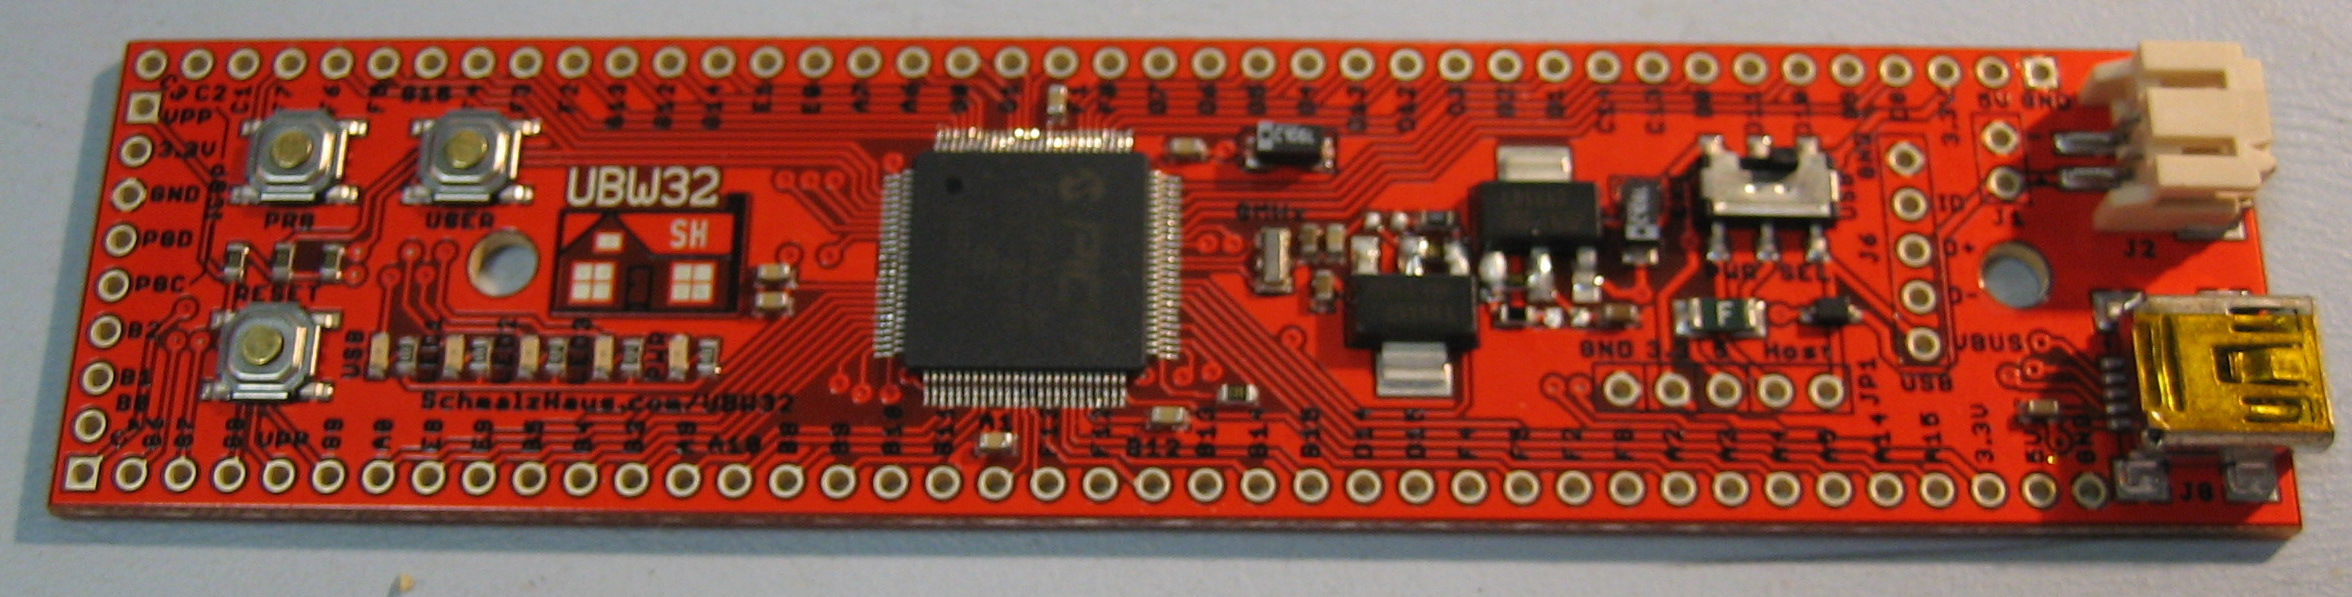
\includegraphics[width=0.75\textwidth]{figures/UBW32_v24_SparkFun.JPG}
  \caption{UBW32 board from SparkFun electronics\protect\cite{Schmalz2013}}
  \label{ubw32fig}
\end{figure}

\paragraph{PICKIT3}A hardware programmer for the PIC32MX795F512L
microprocessor. See figure \ref{pickit3fig}. The pickit3 and program and debug
the PIC32 micro-controller.  Used to download code onto the UBW32. Useful for
installing new bootloaders onto the UBW32 and for restoring broken
firmware\cite{pickitdata}.

\begin{figure}
  \centering
    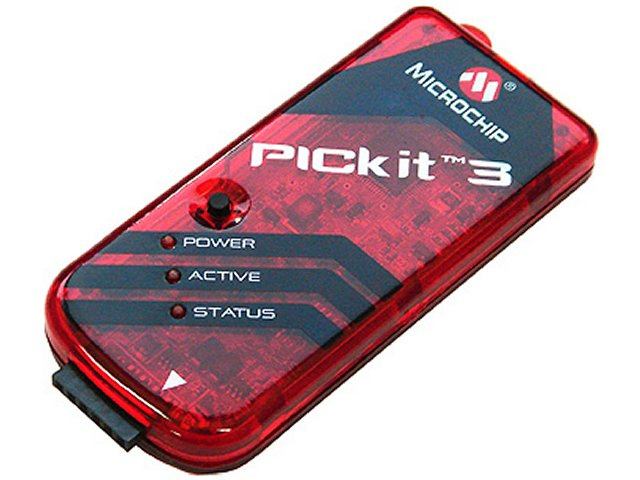
\includegraphics[width=0.3\textwidth]{figures/pickit3.jpg}
  \caption{PICkit 3 In-Circuit Debugger from Microchip\protect\cite{pickitfigcite}}
  \label{pickit3fig}
\end{figure}

\paragraph{MPU6050}A gyro and accelerometer for obtaining information about the
kinematics of the arm and the leg. See figure \ref{mpufig}. Uses I2C connection
to the PIC32MX795F512L for communication\cite{mpu6050data}.

\begin{figure}
  \centering
    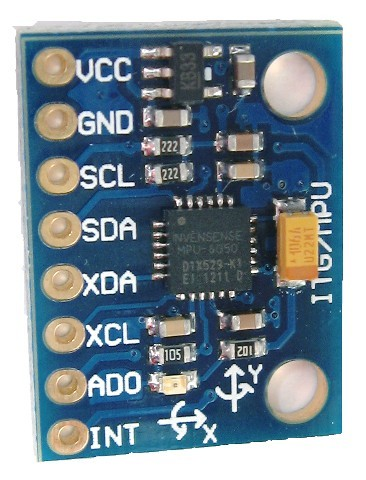
\includegraphics[width=0.2\textwidth]{figures/mpu-6050.jpg}
  \caption{MPU-6050 Triple axis accelerometer and gyro\protect\cite{Krodal2013}}
  \label{mpufig}
\end{figure}

\paragraph{HSR-5498SG}Servos from Hitec. Utilized to control arm and leg
joints. See figure \ref{hsrfig}. The servos require 6-7 Volts. Each servo
requires at least 200mA when running without load, and over 1A when stalled.
The actuation of the arm is accomplished by mini-motors rather than
servos\cite{sscdata}.

\begin{figure}
  \centering
    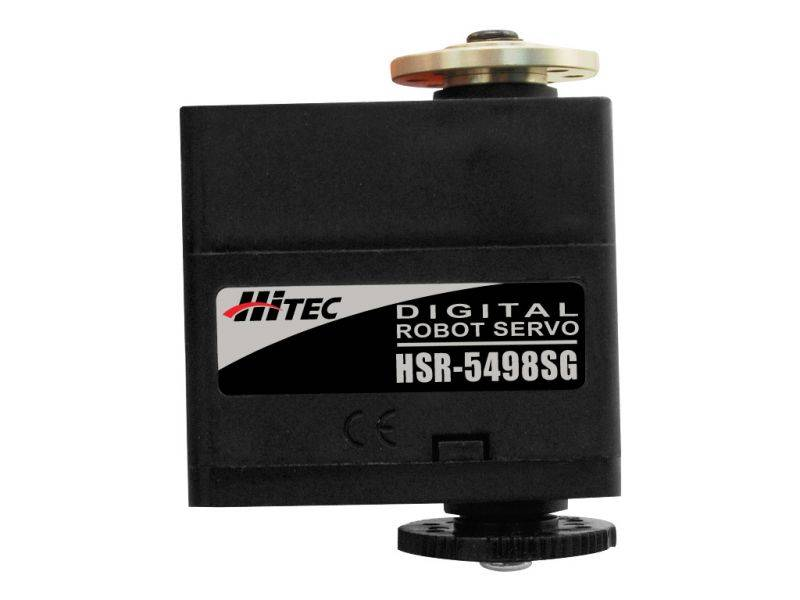
\includegraphics[width=0.4\textwidth]{figures/191_1_HSR-5498SG_HMI_Premium_Robot_Servo-1.jpg}
  \caption{HSR-5498SG servo from Hitech\protect\cite{hsrfigcite}}
  \label{hsrfig}
\end{figure}

\paragraph{SSC-32}Servo controller from Lynx motion. The on-board controller is
an Atmega168-20PU. See figure \ref{sscfig}. The SSC-32 is controlled using
serial signals from another microprocessor or the PC. The control signal is a
string containing a series of commands. The controller can specify pin number,
servo position, rotation speed, and rotation time. It can power 32 servos
simultaneously\cite{servodata}.

\begin{figure}
  \centering
    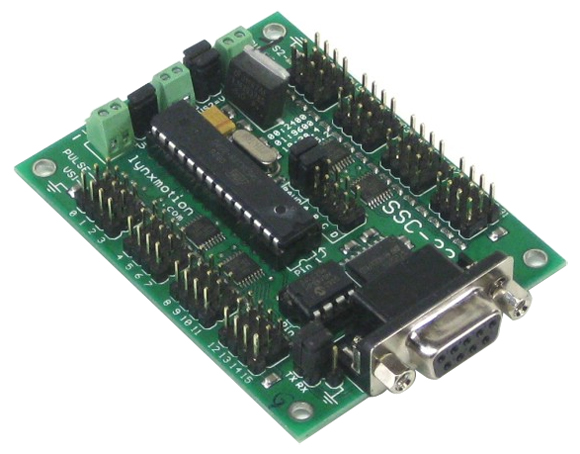
\includegraphics[width=0.4\textwidth]{figures/lynxmotion-ssc-32-servo-controller-large.jpg}
  \caption{SSC-32 servo controller from Lynxmotion\protect\cite{sscfigcite}}
  \label{sscfig}
\end{figure}

\paragraph{VLT100-4002}Power supply for powering the servos. See figure
\ref{vltfig}. 5V output capable of supplying 3A to 12A of current\cite{vltdata}.

\begin{figure}
  \centering
    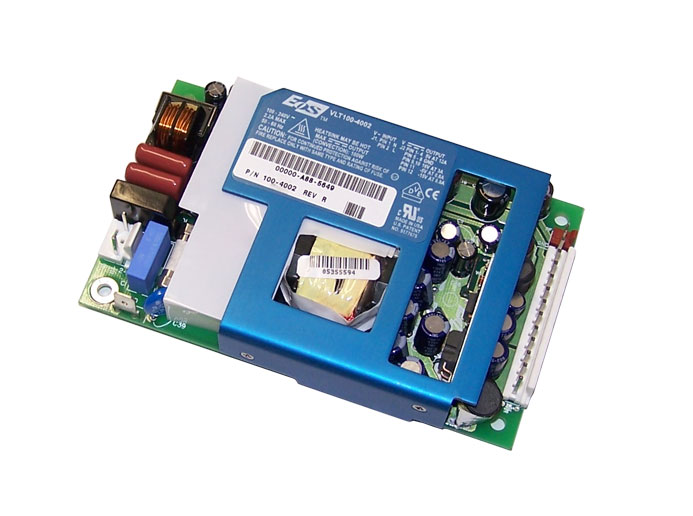
\includegraphics[width=0.4\textwidth]{figures/VLT100-4002.jpg}
  \caption{VLT100-4002 power supply\protect\cite{vltfigcite}}
  \label{vltfig}
\end{figure}

\paragraph{Yihua 1502DD}Adjustable power supply for servos. See figure
\ref{yihuafig}. 0-15V output and 0-2A output\cite{yihuadata}. 

\begin{figure}
  \centering
    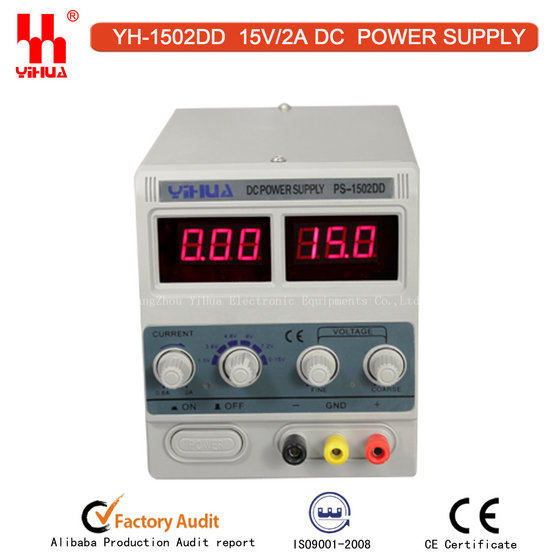
\includegraphics[width=0.4\textwidth]{figures/Power_Supply_YIHUA_1502DD.jpg}
  \caption{Yihua 1502DD DC power supply\protect\cite{yihuafigcite}}
  \label{yihuafig}
\end{figure}

\subsection{Methods}
\subsubsection{Microcontroller Setup}
\paragraph{}To program the PIC32MX795F512L, we used the Multi-Platform
Integrated Development Environment(MPIDE) from chipKIT. To use MPIDE
with the program, we had to program the PIC32 with the avrdude bootloader found
here: \url{https://github.com/chipKIT32/PIC32-avrdude-bootloader}. Using the
PICkit3, we loaded the new bootloader onto the UBW32 and was able to use MPIDE
to program the board. MPIDE utilizes the Arduino libraries and Arduino style C++
code for programming the board. Through MPIDE, there are a wide variety of
libraries available for performing basic I/O tasks using the PIC32.

\subsubsection{MPU-6050 Setup}
\paragraph{}The MPU-6050 utilizes an I2C connection to the read and write data.
The device readings are stored on a 1024 byte FIFO buffer on the
MPU\cite{mpu6050data}. The MPU can be used to acquire sensory information for
controlling the motions of the legs and the arms. We set up the MPU6050 using
the PIC32 I2C libraries in MPIDE. We utilized the \verb!Wire.h! library to read
and write to the I2C bus of the PIC32\cite{Krodal2013}. There are a total of
five SDA pins on the PIC32MX795F512L, so we can have a minimum of five of these
devices connected to our microcontroller.

\subsubsection{Servo Setup}
\paragraph{}The servos each had a range of 180 degrees. The SSC-32 represents
this as a value between 500 and 2500. Due to the mechanical construction most
joints had a limited range of motion. Most joints had a range of 100 degrees.
The exact ranges were tested and calibrated after the completion other robot
leg. Each servo requires approximately 6V and 200mA to 1A of current depending
on the load\cite{servodata}. For our tests, we used the Yihua DC power supply
which is adjustable up to 15V and supplied up to 2A\cite{yihuadata}.

\subsubsection{Servo Control}
\paragraph{}To control the servos we utilized a SSC-32 servo controller. The
controller has 32 channels for servo control. Each channel can be given a
position, rotation speed, and rotation time. Multiple servo channels can be
controlled simultaneously through a single command The SSC-32 is powered through
a 9V battery. The controls are given in the form of strings, the following is an
example of the commands used for SSC-32.
\begin{verbatim}
#5 P1600 T1000 <cr>
\end{verbatim}
The \#5 defines the channel number which ranges from 0 to 31. The P1600 sets the
position of the servo from 500 to 2500. The T1000 sets the time of rotation in
milliseconds. The carriage return(\verb!<cr>!) signifies the completion of a
command. The following is an example command for simultaneous movement of
servos:
\begin{verbatim}
#5 P1600 #10 P750 T2500 <cr>
\end{verbatim}
In this case all the servos adjust their speed so they arrive at the specified
position in the specified time.

\subsubsection{Walking Algorithm Implementation}
\paragraph{} The walking algorithms were designed by Zhu Ziqi, a fellow team
member. He designed and simulated the algorithms in MATALB and SIMULINK and I
implemented the algorithms in C++ on the PIC32MX795F512L. The servo positions
were determined from a linear combination of sine waves. For our preliminary
walking algorithms we only considered the knee and hip joints. The SSC-32
position control signal requires a integer ranged from 500 to 2500,
corresponding to $180^{\circ}$ of motion\cite{sscdata}. Due to the mechanical
construction of the arm and leg joints, which mimicked human structure, most
joint servos were limited to a range between 1250 and 2500. The output from the
sine waves would be converted to a range in the SSC-32's output and then sent to
the servos. Equations \ref{thetahip} and \ref{thetaknee} show the equations for
calculating the position of each servo as a function of time. The angle of the
hip is a degree relative to the vertical axis of the 3D space, while the angle
of the knee is relative to the axis along the thigh of the robot.
\begin{align}
    \phi_{3}(t)&=a_{13L}sin(b_{13L}t+c_{13L})+a_{23L}sin(b_{23L}t+c_{23L})+a_{33L}sin(b_{33L}t+c_{33L})\nonumber\\
    &+a_{43L}sin(b_{43L}t+c_{43L})+a_{53L}sin(b_{53L}t+c_{53L})+a_{63L}sin(b_{63L}t+c_{63L})\nonumber\\
    &+a_{73L}sin(b_{73L}t+c_{73L})+a_{83L}sin(b_{83L}t+c_{83L}) \label{phi3}\\
    \phi_{4}(t)&=a_{14L}sin(b_{14L}t+c_{14L})+a_{24L}sin(b_{24L}t+c_{24L})+a_{34L}sin(b_{34L}t+c_{34L})\nonumber\\
    &+a_{44L}sin(b_{44L}t+c_{44L})+a_{54L}sin(b_{54L}t+c_{54L})+a_{64L}sin(b_{64L}t+c_{64L})\nonumber\\
    &+a_{74L}sin(b_{74L}t+c_{74L}) \label{phi4}\\
    \theta_{hip}(t)&=\frac{\phi_{3}(t)}{180\pi} \label{thetahip}\\
    \theta_{knee}(t)&=\frac{\theta_{hip}(t)-\phi_{4}(t)}{180\pi} \label{thetaknee}\\
\end{align}
The conversion from angle in degrees to servo position is given by the following
equation.
\begin{align}
    P=\frac{\theta}{90}*1000+1500
\end{align}
The positions of the legs are calculated by the PIC32 and sent to the SSC-32
through the Universal Asynchronous Receiver Transmitter(UART) module of the
PIC32. The UART is a serial connection between the PIC32 and the SSC-32. The
calculated results are composed into a string in the form of an SSC-32 command
and sent to the servo controller. 

\section{Discussion}
\subsection{Overall System}
\paragraph{}Currently we have components of a robotic platform prototyped and
designed. The Robotic legs and arm are prototyped and constructed. The hand and
feet have been designed in CAD, and The basic software and control framework has
been established. The basic I/O and control tasks have been implemented in C++
on the microcontroller with easy to use APIs that others can use to control the
currently completed robot legs. Overall we are at a good position for the
sponsor to take the foundations we have built and try to implement different
control algorithms and machine learning algorithms. 

\subsection{Robot Leg}
\paragraph{}The leg was constructed using with six servos on each leg. Three
servos on the hip mimicked the ball and socket configuration of the human hip
joint, which has three degrees of freedom\cite{SiasJr1990}. The three modes of
motion are along the sagittal, frontal, and transverse planes\cite{Fiscell2005}.
The knee has one degree of freedom, and the ankle has two degrees of freedom in
the sagittal and frontal planes. Each leg has six degrees of freedom in total,
this is fine for most gaits on uneven ground, but more complex terrain may be 
difficult to manage; More degrees of freedom may be needed to obtain more human
like gait on difficult to traverse terrains\cite{SiasJr1990}.

\paragraph{}The shins and pelvis were constructed from aluminum U channels. The
thighs where made from aluminum cylinders, and the feet were aluminum plates
(Figure \ref{protolegfig}). The SSC-32 servo controller was attached to the hip.
A tether connects the servo controller to the power supply and the PIC32
controller. Figure \ref{servosetupfig} shows the configuration of the servos on the leg, as
well as their direction and range of motion in terms of SSC-32 position values.

\begin{figure}
  \centering
    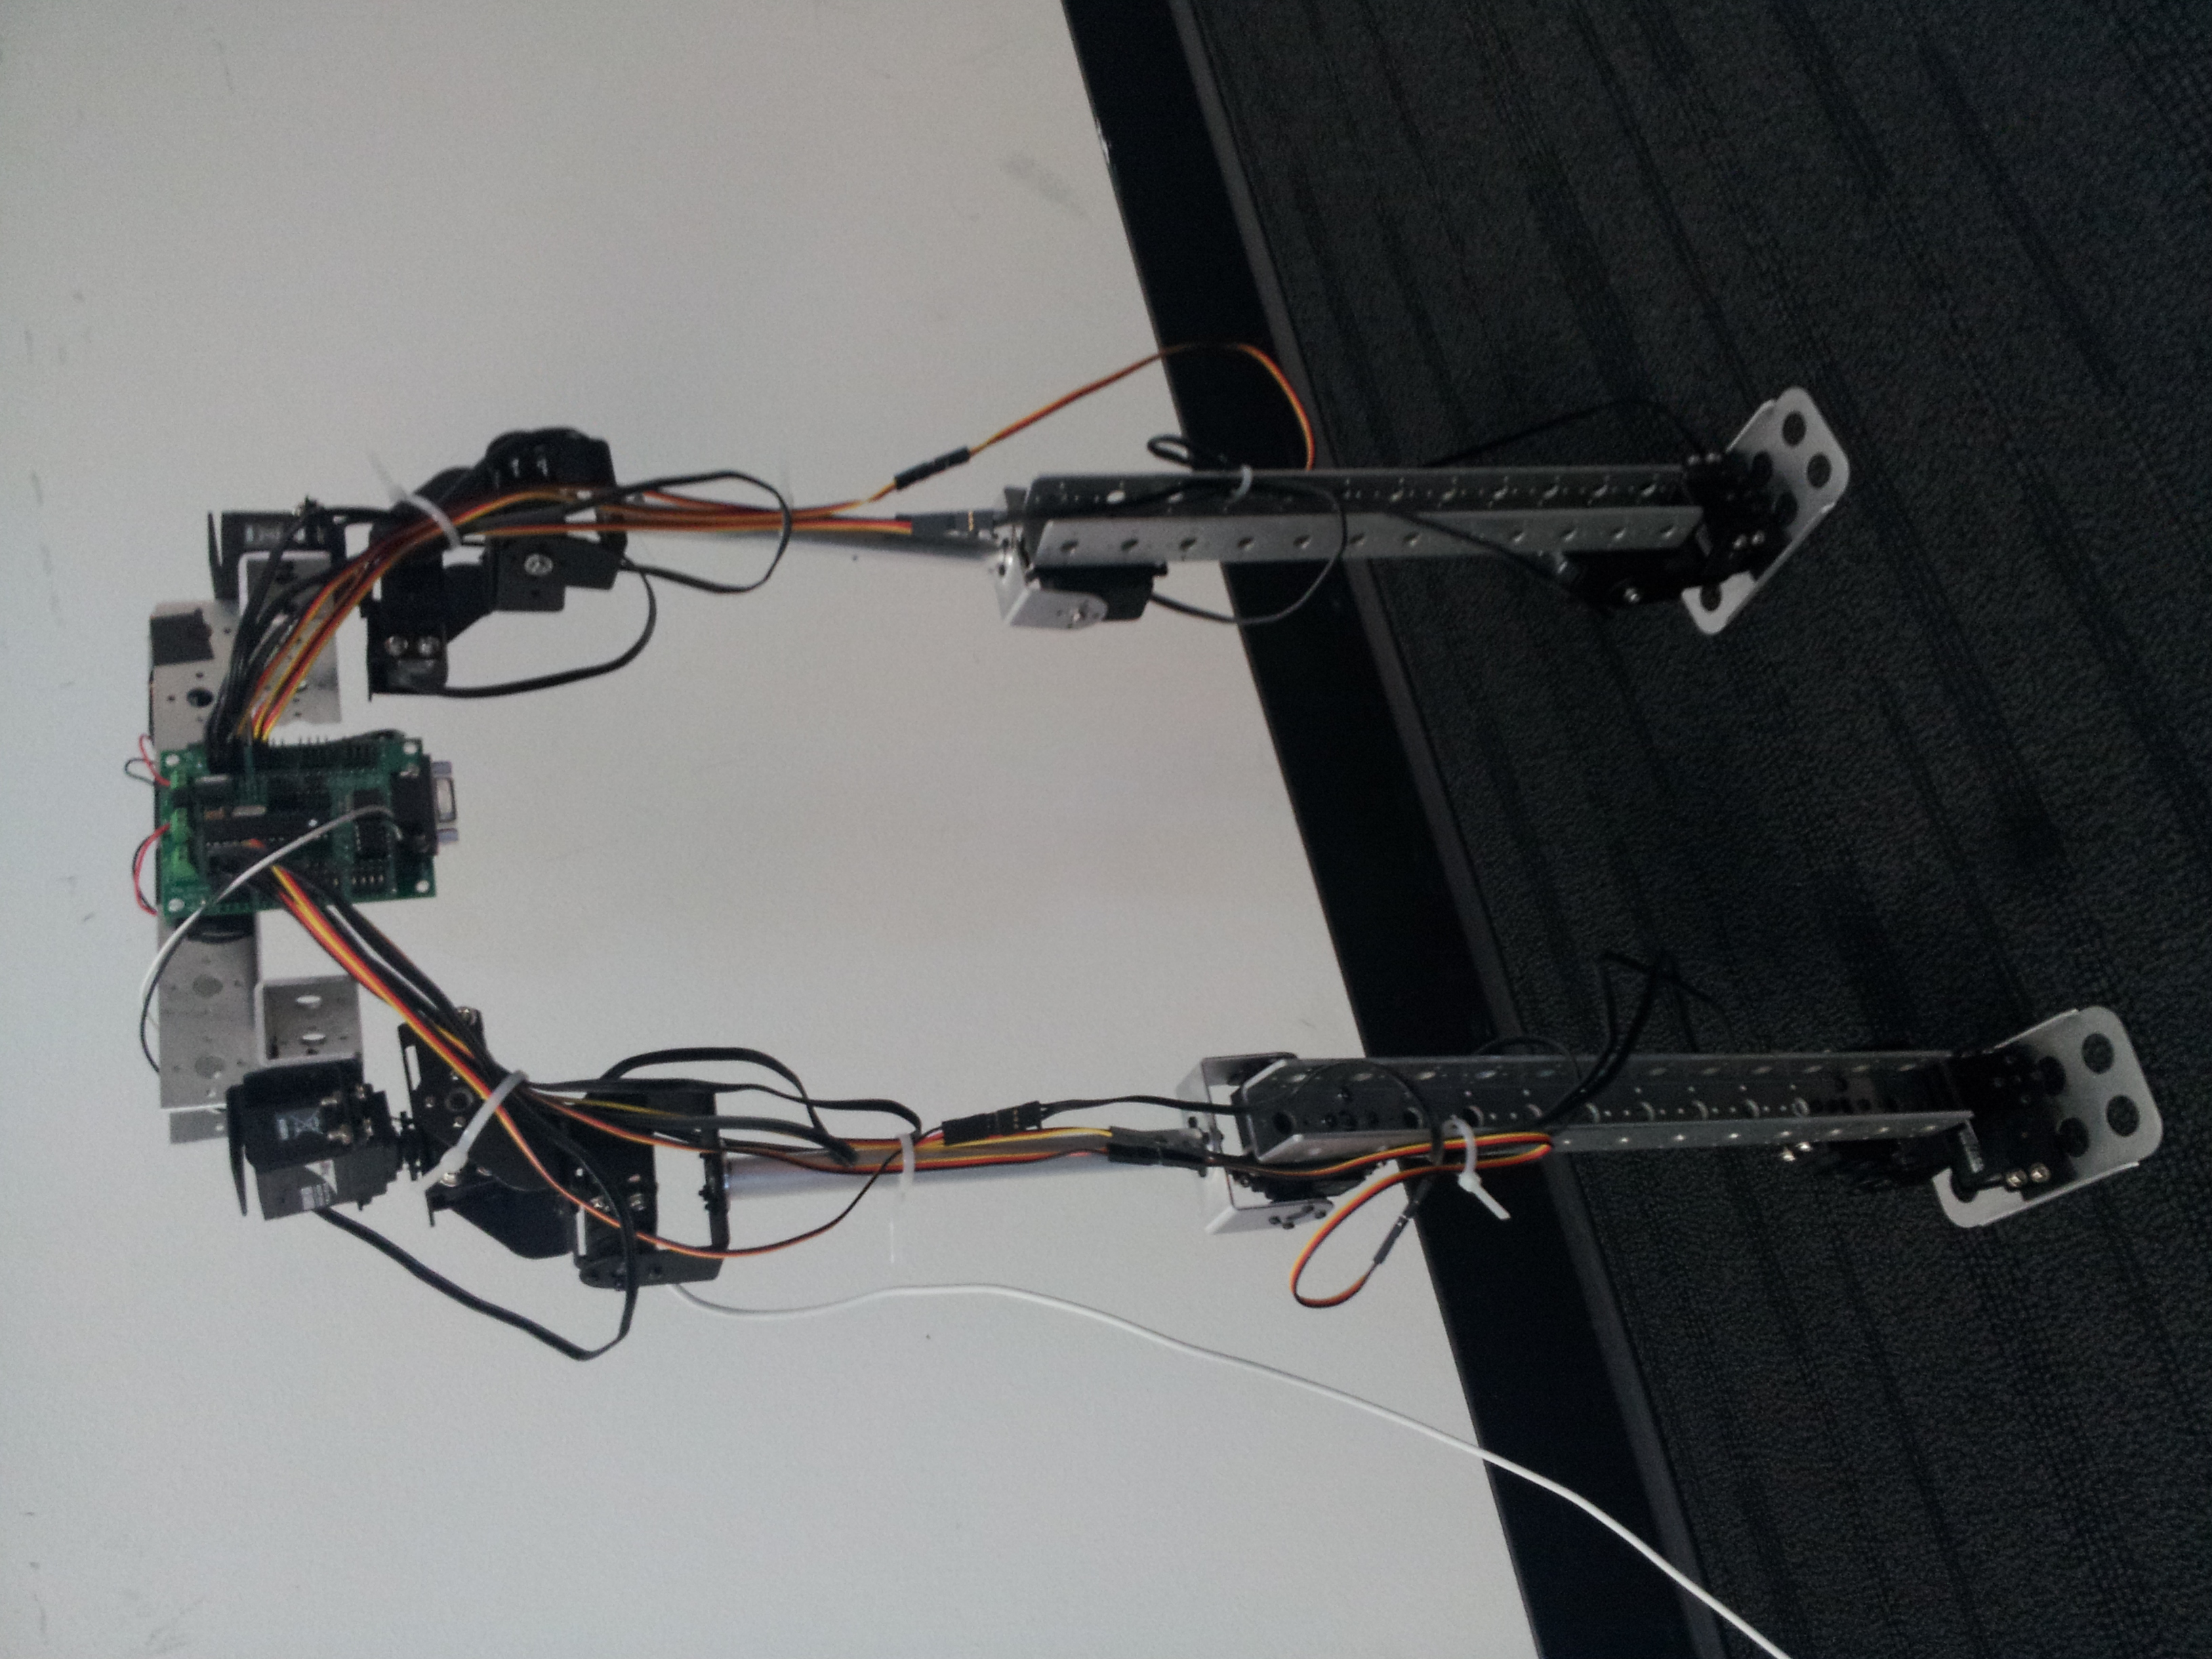
\includegraphics[width=0.7\textwidth,angle=270]{figures/LegPrototype.jpg}
  \caption{Prototype leg constructed of aluminum. Total of 6 degrees of freedom
  on each leg. The servo controller is attached to the hip}
  \label{protolegfig}
\end{figure}

\begin{figure}
  \centering
    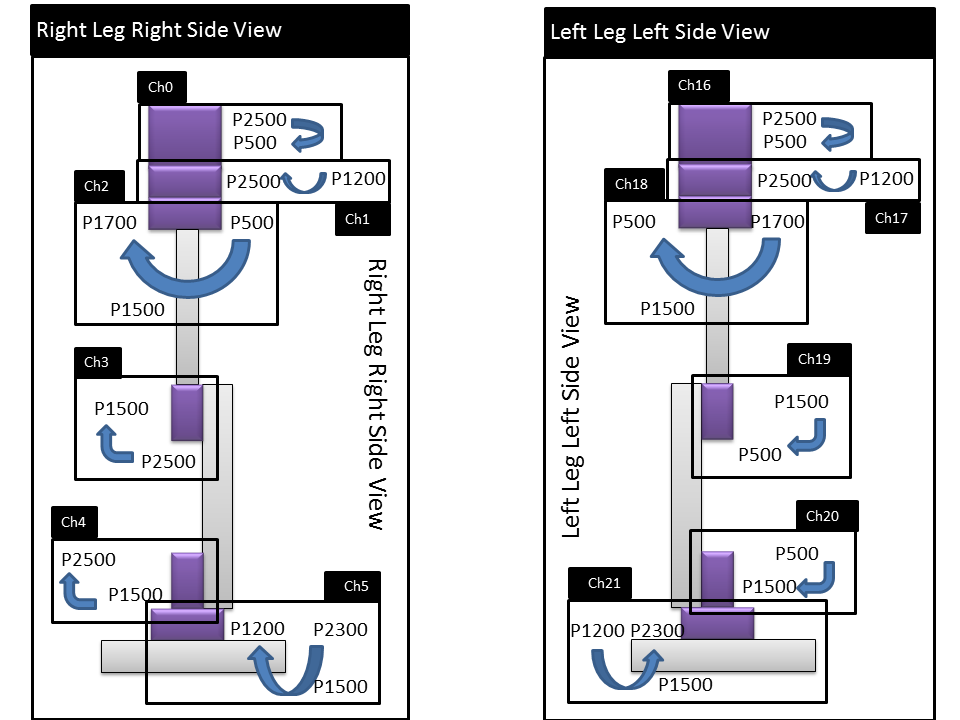
\includegraphics[width=1.0\textwidth]{figures/LegConfiguration.png}
  \caption{Location of the servos on the leg, and the directions and ranges of
  motion for each servo in terms of the SSC-32 position outputs}
  \label{servosetupfig}
\end{figure}

\subsection{Firmware}
\paragraph{}The currently completed firmware components are the serial
communications to different devices, servo control, and accelerometer/gyro
control.  The communications channels implemented are the USB communications
between the PIC32 and the PC, the UART connection between the PIC32 and the
SSC-32 servo controller, and the I2C connection to the MPU6050 sensors. The I2C
connection can be adapted to more sensors that may be added in the future for
other devices. 

\paragraph{}The servo controls are accessed through \verb!SSCServo.h! which
contains functions and settings for controlling servo position through the
SSC-32 controller. The MPU6050 is accessed through \verb!MPU6050.h! which
defines memory addresses of the MPU6050 registers and functions for reading the
output of the sensors and configuring the sensor settings. Future users of the
robot can adapt these settings to program and prototype their own control
algorithms.

\subsection{Locomotion Controller}
\paragraph{}Ziqi performed the simulations of the robot leg locomotion
algorithms, and obtained the optimal parameters for equations \ref{phi3} and
\ref{phi4}. The following are the parameters we used. Refer to Ziqi's report for
a detailed analysis of the control system.
\begin{verbatim}
phi_3:           phi_4:
a13L =   73.11;  a14L =  14.91;
b13L =   19.69;  b14L = 0.8727;
c13L = -0.6449;  c14L =  4.016;
a23L =   52.58;  a24L =  1.559;
b23L =  0.6307;  b24L =   19.4;
c23L =   2.671;  c24L = -1.197;
a33L =   12.35;  a34L =  27.52;
b33L =   12.05;  b34L =  15.42;
c33L =  -2.836;  c34L = 0.9818;
a43L =   3.357;  a44L =  28.88;
b43L =   29.81;  b44L =  45.43;
c43L =  -0.797;  c44L = -5.819;
a53L =   62.63;  a54L =  15.08;
b53L =   20.15;  b54L =  31.49;
c53L =   2.236;  c54L =  1.844;
a63L =   12.04;  a64L =  1.769;
b63L =   5.405;  b64L =  9.852;
c63L =   3.598;  c64L = -5.219;
a73L =   1.786;  a74L =   31.1;
b73L =   34.76;  b74L =  45.58;
c73L =   1.995;  c74L = -2.751;
a83L =   1.418;
b83L =    47.2;
c83L =  -0.402;
\end{verbatim}

\paragraph{}The robot is controlled through a serial connection to the computer.
The PIC32MX795F512L is connected to the PC through the USB connection on UART
channel 0. Commands can be passed into the robot from a serial terminal on the
PC. Currently there are three modes of operation: Standing, Walking, and Direct
Control. Activated by sending the strings \verb!stand!, \verb!walk!, and
\verb!direct! through a serial terminal to the PIC32. While in stand mode, the
robot holds a rigid upright position. While in walk mode, the robot attempts to
walk according to the sine waves laid out by equations \ref{phi3} to
\ref{thetaknee}. In direct mode, each servo can be commanded directly using
the SSC-32 commands; in this mode all the commands passed to the PIC32 are
redirected to the SSC-32. Servos on the right leg are attached to channels 0-5
on the SSC-32 and the servos on the left leg are on channels 16-21. Figure
\ref{servosetupfig} shows the corresponding channels for each servo.

\subsection{System Analysis}
\paragraph{}The controller runs performs simple round robin scheduling when
calculating servo outputs. It looks at each servo in order and calculates the
correct output. The final command is composed from the servo outputs and sent as
a single synchronized motion command to the SSC-32. The execution speed of the
round robin loop is determined in the code. To get smooth motions in the joints,
we needed to calibrate the timing of the commands sent to the SSC-32. Currently
we are utilizing a 100ms time step for the position calculations, and we found
that approximately 90ms update time is sufficient for smooth motions. We
calculate the necessary position of the servos and construct the command and
send the command to the SSC-32 in 90ms. Currently we have 12 servos, and each
servo requires around 8 bytes of data to be sent.  The PIC32 runs at 80Mhz, so
it is sufficient for our current configuration \cite{pic32data}. The serial
transfer rate can be limiting since the SSC-32 requires a long string encoding
the positions of all the servos that need to be moved, and each servo needs a
string of 8 characters, with 12 servos on the legs and 12 servos on the arms
that is 1536 bits of information that needs to sent every time step. However the
SSC-32 has a maximum baud rate of 115.2kbps, so we cant send that information in
approximately 13ms \cite{sscdata}. Equation \ref{transfertime} shows the bit
rate calculations.
\begin{align}
    t_{serial} &= \frac{n_{servos} * \frac{8 bytes}{servo} * \frac{8 bits}{byte}}
        {115.2 kbps} \label{transfertime}
\end{align}
The maximum update speed for the SSC-32 is 20ms, so that is the main performance
limiter \cite{lynxmaxspeed}.  The 20ms limit should be fine for most motions,
since 20ms is faster than most human knee motions
\cite{williamson2001detecting}. However, having a faster update rate will
increase the resolution of the motion and achieve a more human like gait.The
SSC-32 is controlled by a Atmel ATMEGA168-20PU, which is a 8-bit 20Mhz
microcontroller \cite{Atmega168data}. To increase performance, we may be able
to shift the servo control to the PIC32, which is a much faster microcontroller,
and we would not need the serial communications between the PIC32 and the
SSC-32, but that would require more complicated task scheduling to synchronize
the servo movements.

\paragraph{}Currently, the motion of the legs is restricted due to lack of
proper power supply to the robot. Currently we only have two power supplies, the
Yihua 1502DD and the VLT100, neither of which is suitable for the task of
powering the entire bipedal system. Currently the Yihua can support full control
of a single joint with great reliability. The datasheet of the servos list the
stall current as 1.2A and the no load current as 200mA. Through testing we see
that actuating a single knee servo to lift the leg requires over 1A of current.
The Yihua has a maximum load of 2A, which cannot support motion of the robot.
Testing with the VLT100 which is a 5V 3-12A power supply also proved useless.
The power supply could no reliably lift the legs of the robot and hold their
positions. The leg has 12 servos in total, most of large motions will be in the
four hip and knee joints, while the other joints will be responsible for smaller
motions to balance the robot. The arms are of similar construction, but the
elbow and shoulder joints would be responsible for a even larger load of lifting
the arms in air. 

\paragraph{}Ideally we want to be able to supply 28.8A of current to
satisfy the maximum requirement of the servos. We can opt for a high current
power supply such as a BK Precision Model 1796, which can supply 0-16V and 0-50A
which will be enough for our applications \cite{bkpowerdata}. However such
supplies are probably too bulky to be put on to the robot chassis, so the robot
will need to be tethered to the table supply. We can also boost the voltage out
put of the VLT100, the 12A output is probably sufficient for the controlling the
legs or the arms, so we may need two supplies for the whole robot. The VLT100 is
small enough to attach to the robot, but it needs to be attached to tethered to
the wall supply. We can also use batteries to power the robot. The BP13-6 S for
BB Battery Co. has 6V output and a 30A maximum discharge, and the battery is
rechargeable \cite{batterydata}. The battery has the advantage of being mobile
and can remove the necessity of tethering the robot, though the battery is
fairly heavy at 5.5lb \cite{batterydata}. To fully free the robot from the
tether, we will also need to replace the wired USB connection with wireless
communication.

\section{Conclusion}
\paragraph{}Currently the robot has legs and arms that can be used as testing
platforms for various algorithms. Future groups can utilize this robotic
platform as a foundation for developing more complex control systems and
artificial intelligence software. The overall vision laid out by the our
industry adviser at the beginning of the project was of a humanoid robot that
has advanced locomotion capabilities such as running and jumping and advanced
vision and hand manipulation capabilities. The goal for our group was to build
the foundations of this robot. We have successfully prototyped the simpler
components like the leg and arm, and we have laid the software foundations for
the control system and computer vision system. It would be easy for future teams
to build on the software and hardware we have to complete the vision of our
sponsor.

\paragraph{}More testing and simulations need to be done to finish the control
systems of the robot. More degrees of freedom can also be added to implement
more human like motions. Once that is completed more work can be done to push it
beyond the state of the art, by implementing complex motions such as bipedal
running. The vision system needs to be completed and interfaced to the robot
arm, so the vision can be used to guide the arm's motions. We faced difficulties
in the mechanical design of the hand with the constraints of size and weight,
especially in implementing SMA into the design, so more work and testing need to
be done in this area.

\paragraph{}The areas of advanced robotic locomotion, computer vision, and
advanced humanoid hand and feet design are all great areas for the sponsor Bay
Area IP to explore IP opportunities. These technologies can bring many benefits
to areas such as manufacturing and prosthetics.

\clearpage
\printbibliography

\end{document}
